
\chapter{Object Detection}

Usually, there are often multiple objects in the image of interest.
We not only want to know their categories, but also their specific positions in the image.
In computer vision, we refer to such tasks as object detection (or object recognition).


\section{Single-Shot Detector}
\label{sec:single-shot-detector}



The object dection model used here is the SSD\footnote{\url{https://arxiv.org/pdf/1512.02325.pdf}}.

The code is on \href{https://github.com/mingmingli916/object_detection_pytorch}{Github}.


Figure \ref{fig:sd} show the structure.
\begin{figure}[!htbp]
  \centering
  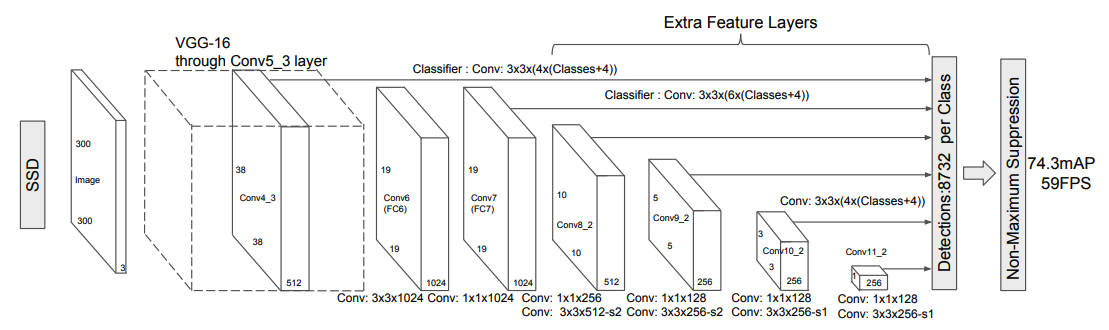
\includegraphics[width=0.9\textwidth]{ssd}
  \caption{SSD}
  \label{fig:ssd}
\end{figure}

There are two parts: backbone and SSD head.
The backbone is the EGG as the feature extractor.
The SSD head is a set of convolution layers.
The SSD head extracts features on different size.
Then it do regression and classification to achieve anchor box offset and object class.

\subsection{Bounding box}
\label{sec:bounding-box}


In object detection, we usually use a \keyword{bounding box} to describe the spatial location of an object.
The bounding box is rectangular, which is determined by the $x$ and $y$ coordinates of the upper-left corner of the rectangle and the such coordinates of the lower-right corner.
Another commonly used bounding box representation is the $(x, y)$-axis coordinates of the bounding box center, and the width and height of the box.

For example in Figure \ref{fig:bounding-box}.
\begin{figure}[!ht]
  \centering
  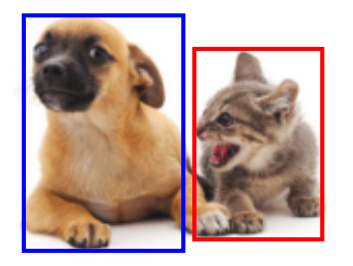
\includegraphics[width=0.7\textwidth]{bounding-box.png}
  \caption{Bounding box}
  \label{fig:bounding-box}
\end{figure}



\subsection{Anchor boxes}
\label{sec:anchor-boxes}

Object detection algorithms usually sample a large number of regions in the input image, determine whether these regions contain objects of interest, and adjust the boundaries of the regions so as to predict the ground-truth bounding boxes of the objects more accurately.

Different models may adopt different region sampling schemes.
One method is: it generates multiple bounding boxes with varying scales and aspect ratios centered on each pixel.
These bounding boxes are called \keyword{anchor boxes}. 



Suppose that the input image has a height of $h$ and width of $w$.
We generate anchor boxes with different shapes centered on each pixel of the image.
Let the scale be $s \in (0, 1]$ and the aspect ratio (ratio of width to height) is $r > 0$.
Left out the scale $s$ and the anchor box area does not change.
The new width and height of the anchor box are $w\sqrt{r}$ and $h/\sqrt{r}$ respectively.
Counting the scale $s$, those are $ws\sqrt{r}$ and $h/\sqrt{r}$ respectively.
Note that when the center position is given, an anchor box with known width and height is determined.


To generate multiple anchor boxes with different shapes, let us set a series of scales $s_{1}, \dots, s_{n}$ and a series of aspect ratios $r_{1}, \dots,r_{m}$.
When using all the combinations of these scales and aspect ratios with each pixel as the center, the input image will have a total of $whnm$ anchor boxes.
Although these anchor boxes may cover all the ground-truth bounding boxes, the computational complexity is easily too high.
In practice, we can only consider those combinations containing $s_{1}$ and $r{1}$:
\begin{equation}
  \label{eq:1}
  (s_{1}, r_{1}), (s_{1}, r_{2}), \dots, (s_{1}, r_{m}), (s_{2}, r_{1}), (s_{3}, r_{1}), \dots, (s_{n}, r_{1})
\end{equation}
That is to say, the number of anchor boxes centered on the same pixel is $n + m - 1$.
For the entire input image, we will generate a total of $wh(n + m - 1)$ anchor boxes.

For example in Figure
\begin{figure}[!ht]
  \centering
  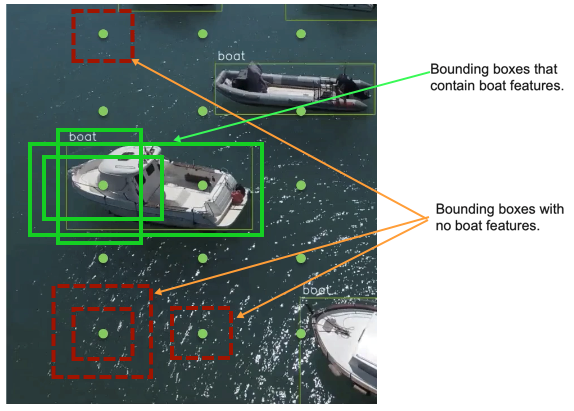
\includegraphics[width=0.8\textwidth]{anchor-boxes.png}
  \caption{Anchor boxes}
  \label{fig:anchor-boxes}
\end{figure}


\subsection{IntersectionoverUnion(IoU)}
\label{sec:iou}

We use IoU to measure the similarity between the anchor boxes and the ground-truth bounding box.


\subsection{Labeling Anchor Boxes in Training Data}
\label{sec:label-anch-boxes}

In a training dataset, we consider each anchor box as a training example.
In order to train an object detection model, we need class and offset labels for each anchor box.


To label any generated anchor box, we refer to the labeled location and class of its assigned ground-truth bounding box that is closest to the anchor box.

Given an image,suppose that the anchor boxes are \(A_{1}, A_{2}, \ldots A_{n_{a}}\) and the ground-truth bounding boxes are \(B_{1},B_{2},\ldots B_{n_{b}}\), where \(n_{a} \ge n_{b}\).
Let us define a matrix \(X \in R_{n_{a}\times n_{b}}\), whose element \(x_{ij}\) in the \(i^{th}\) row and \(j^{th}\) column is the IoU of the anchor box \(A_{i}\) and the ground-truth bounding box \(B_{j}\).
The algorithm consists of the following steps:

\begin{enumerate}
\item \label{item:1}Find the largest element in matrix \(X\) and denote its row and column indices as \(i_{1}\) and \(j_{1}\), respectively. Then the ground-truth bounding box \(B_{j_{1}}\) is assigned to the anchor box \(A_{i_{1}}\). After the first assignment, discard all the elements in the \(i_{1}^{th}\) row and the \(j_{1}^{th}\) column in matrix \(X\).
\item Repeat process \ref{item:1} until all elements in \(n_{b}\) columns in matrix \(X\) are discarded. 
\item Traverse through the remaining \(n_{a} - n_{b}\) anchor boxes. For example, given any anchor box \(A_{i}\), find the ground-truth bounding box \(B_{j}\) with the largest IoU with \(A_{i}\) throughout the \(i^{th}\) row of matrix \(X\), and assign \(B_{j}\) to \(A_{i}\) only if this IoU is greater than a predefined threshold.
\end{enumerate}

\subsection{Labeling Classes and Offsets}
\label{sec:label-class-offs}

Suppose that an anchor box A is assigned a ground-truth bounding box B.
On one hand, the class of the anchor box A will be labeled as that of B.
On the other hand, the offset of the anchor box A will be labeled according to the relative position between the central coordinates of B and A together with the relative size between these two boxes.
Here's a command transformation.
Given the central coordinates of A and B as \((x_{a}, y_{a})\) and \((x_{b},y_{b})\), their widths as \(w_{a}\) and \(w_{b}\), and their heights as \(h_{a}\)a nd \(h_{b}\), respectively.
We label the offset of A as:
\begin{equation}
  \label{eq:2}
  \bigl(
  \frac{\frac{x_{b}-x_{a}}{w_{a}}-\mu_{x}}{\sigma_{x}},   \frac{\frac{y_{b}-y_{a}}{h_{a}}-\mu_{y}}{\sigma_{y}},
  \frac{\log\frac{w_{b}}{w_{a}}-\mu_{w}}{\sigma_{w}},  \frac{\log\frac{h_{b}}{h_{a}}-\mu_{h}}{\sigma_{h}}
  \bigr)
\end{equation}
where default values of the constants are \(\mu_{x}=\mu_{y}=\mu_{w}=\mu_{h}=0, \sigma_{x}=\sigma_{y}=0.1\) and \(\mu_{w}=\mu_{h}=0.2\).




\section{R-CNN models}

\subsection{Region-based CNN (R-CNN)}
\label{sec:region-based-cnn}

The R-CNN consists of the following four steps:
\begin{enumerate}
\item Perform \keyword{selective search} to extract multiple high-quality \keyword{region proposals} on the input image.
  These proposed regions are usually selected at multiple scales with different shapes and sizes.
  Each region proposal will be labeled with a class and a ground-truth bounding box.
\item Choose a pretrained CNN and truncate it before the output layer.
  Resize each region proposal to the input size required by the network, and output the extracted features for the region proposal through forward propagation.
\item Take the extracted features and labeled class of each region proposal as an example.
  Train multiple \keyword{support vector machines} to classify objects, where each support vector machine individually determines whether the example contains a specific class.
\item Take the extracted features and labeled bounding box of each region proposal as an example.
  Train a \keyword{linear regression} model to predict the ground-truth bounding box.
\end{enumerate}

\begin{figure}[H]
  \centering
  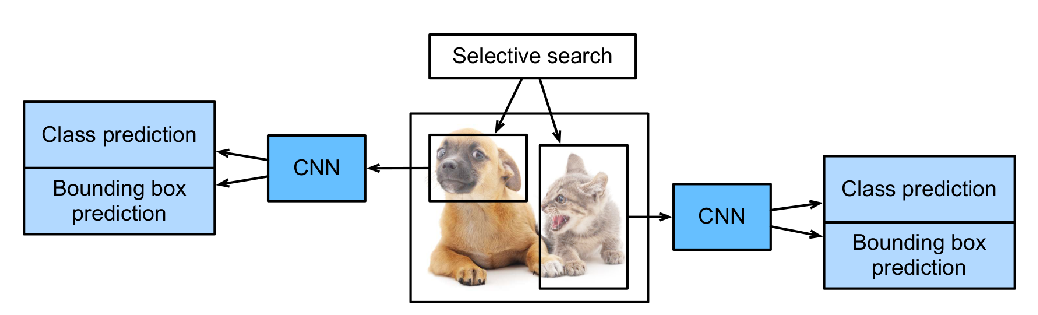
\includegraphics[width=0.8\textwidth]{rcnn}
  \caption{R-CNN}
  \label{fig:r-cnn}
\end{figure}

Although the R-CNN model uses pretrained CNNs to effectively extract image features, it is slow.
Imagine that we select thousands of region proposals from a single input image: this requires thousands of CNN forward propagations to perform object detection.
This massive computing load makes it infeasible to widely use R-CNNs in real-world applications.


\subsection{Fast R-CNN}
\label{sec:fast-r-cnn}

The main performance bottleneck of an R-CNN lies in the independent CNN forward propagation for each region proposal, without sharing computation.
Since these regions usually have overlaps, independent feature extractions lead to much repeated computation.
One of the major improvements of the fast R-CNN from the R-CNN is that the CNN forward prop- agation is only performed on the entire image.

\begin{figure}[H]
  \centering
  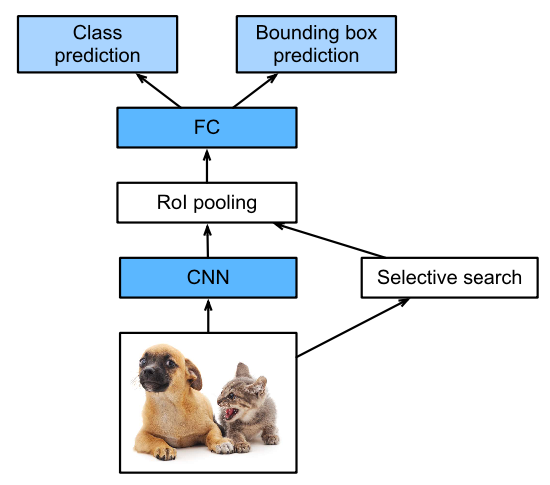
\includegraphics[width=0.8\textwidth]{fast-rcnn}
  \caption{Fast R-CNN}
  \label{fig:fast-rcnn}
\end{figure}

Its major computations are as follows:
\begin{enumerate}
\item Compared with the R-CNN, in the fast R-CNN the input of the CNN for feature extraction is the entire image, rather than individual region proposals.
  Moreover, this CNN is trainable.
  Given an input image, let the shape of the CNN output be \(1 \times c \times h_{1} \times w_{1}\).
\item Suppose that selective search generates n region proposals.
  These region proposals (of different shapes) mark \keyword{regions of interest} (of different shapes) on the CNN output.
  Then these regions of interest further extract features of the same shape (say height \(h_{2}\) and width \(w_{2}\) are specified) in order to be easily concatenated.
  To achieve this, the fast R-CNN introduces the \keyword{region of interest (RoI)} pooling layer: the CNN output and region proposals are input into this layer, outputting concatenated features of shape \(n \times c \times h_{2} \times w_{2}\) that are further extracted for all the region proposals.
\item Using a fully connected layer,transform the concatenated features into an output of shape \(n \times d\), where \(d\) depends on the model design.
\item Predict the class and bounding box for each of the n region proposals.
  More concretely, in class and bounding box prediction, transform the fully connected layer output into an output of shape \(n \times q\) (q is the number of classes) and an output of shape \(n \times 4\), respectively.
\end{enumerate}

\subsection{Faster R-CNN}
\label{sec:faster-r-cnn}

To be more accurate in object detection, the fast R-CNN model usually has to generate a lot of region proposals in selective search.
To reduce region proposals without loss of accuracy, the faster R-CNN proposes to replace selective search with a \keyword{region proposal network}.

\begin{figure}[H]
  \centering
  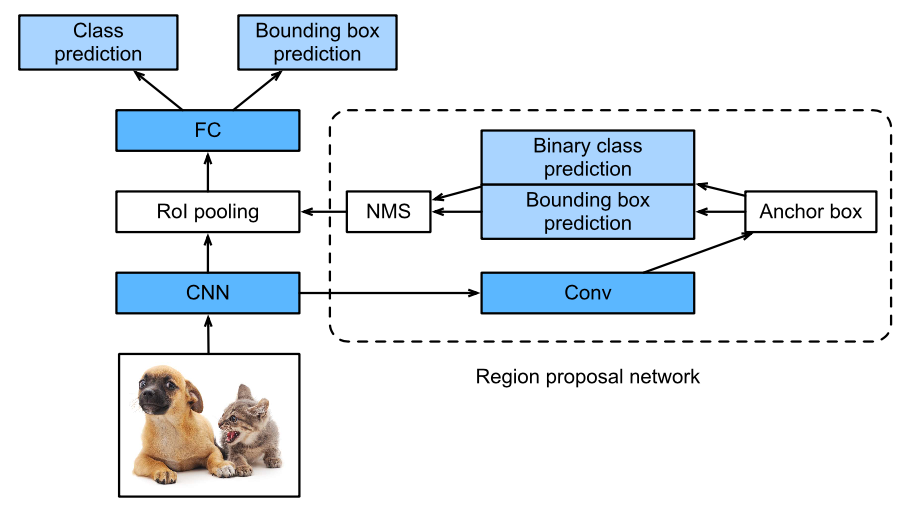
\includegraphics[width=0.8\textwidth]{faster-rcnn}
  \caption{Faster R-CNN}
  \label{fig:faster-rcnn}
\end{figure}

The region proposal network works in the following steps:
\begin{enumerate}
\item Use a \(3 × 3\) convolutional layer with padding of 1 to transform the CNN output to a new output with c channels.
  In this way, each unit along the spatial dimensions of the CNN-extracted feature maps gets a new feature vector of length c.
\item Centered on each pixel of the feature maps, generate multiple anchor boxes of different scales and aspect ratios and label them.
\item Using the length-c feature vector at the center of each anchor box,predict the binary class (background or objects) and bounding box for this anchor box.
\item Consider those predicted bounding boxes whose predicted classes are objects.
  Remove overlapped results using non-maximum suppression.
  The remaining predicted bounding boxes for objects are the region proposals required by the region of interest pooling layer.
\end{enumerate}


\subsection{Mask R-CNN}
\label{sec:mask-r-cnn}

In the training dataset, if pixel-level positions of object are also labeled on images, the mask R-CNN can effectively leverage such detailed labels to further improve the accuracy of object detection.


\begin{figure}[H]
  \centering
  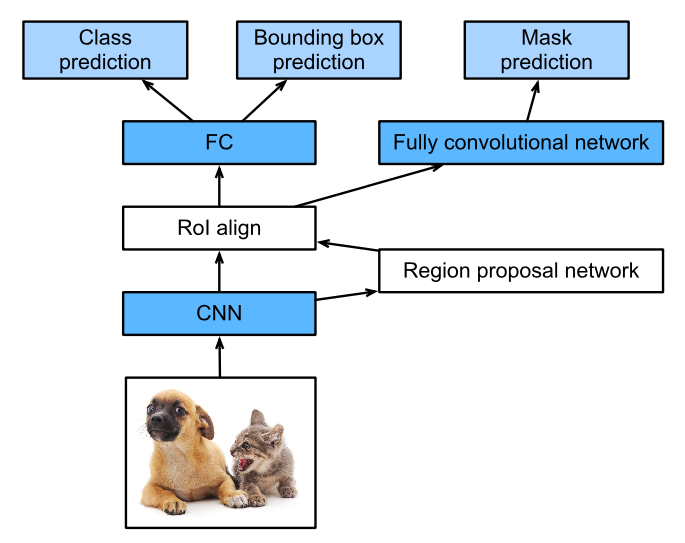
\includegraphics[width=0.8\textwidth]{mask-rcnn}
  \caption{Mask R-CNN}
  \label{fig:mask-rcnn}
\end{figure}

The mask R-CNN replaces the region of interest pooling layer with the \keyword{region of interest (RoI) alignment} layer.
This region of interest alignment layer uses bilinear interpolation to preserve the spatial information on the feature maps, which is more suitable for pixel-level prediction.
The output of this layer contains feature maps of the same shape for all the regions of interest.
They are used to predict not only the class and bounding box for each region of interest, but also the pixel-level position of the object through an additional fully convolutional network.

%%% Local Variables:
%%% mode: latex
%%% TeX-master: "deep-learning"
%%% End:
